\documentclass[professionalfont,10pt]{beamer}
\beamertemplatenavigationsymbolsempty
\addtobeamertemplate{navigation symbols}{}{%
    \usebeamerfont{footline}
    \usebeamercolor[fg]{footline}
    \hspace{5mm}
    \insertframenumber/\inserttotalframenumber
}
\usecolortheme{seahorse}
\setbeamercolor{alerted text}{fg=white!20!blue!30!red}
\setbeamercolor{footline}{fg=black}
\setbeamersize{text margin left=5mm,text margin right=5mm}

\usepackage{graphicx}

\title{How to take action on returned emails in ORSEE}
\author{Lucas Reddinger}
\institute{UCSB}
\date{3 August 2020}

\begin{document}

\frame{\titlepage}

\begin{frame}{An example of a failed email that was returned}
\vspace{0.25cm}
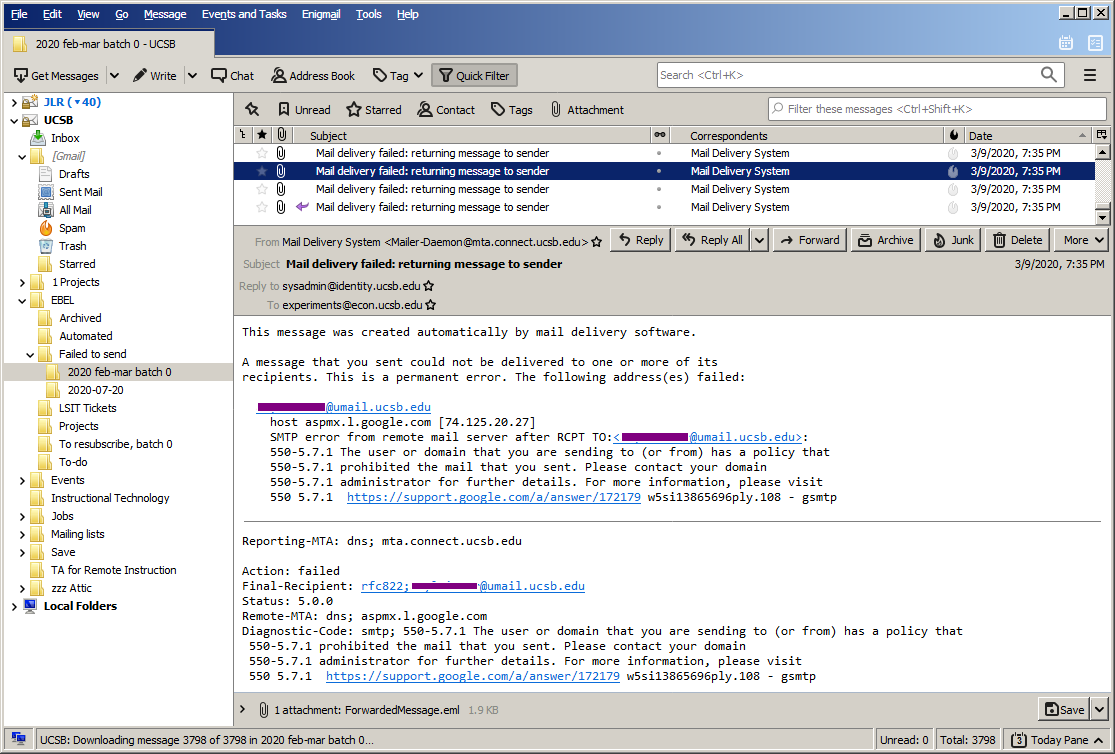
\includegraphics[height=7cm]{email-failed-example.png}
\end{frame}

\begin{frame}{Export emails as a single CSV file}
\begin{itemize}
\item Mozilla Thunderbird using ImportExportTools Add-on
\end{itemize}
\vspace{0.25cm}
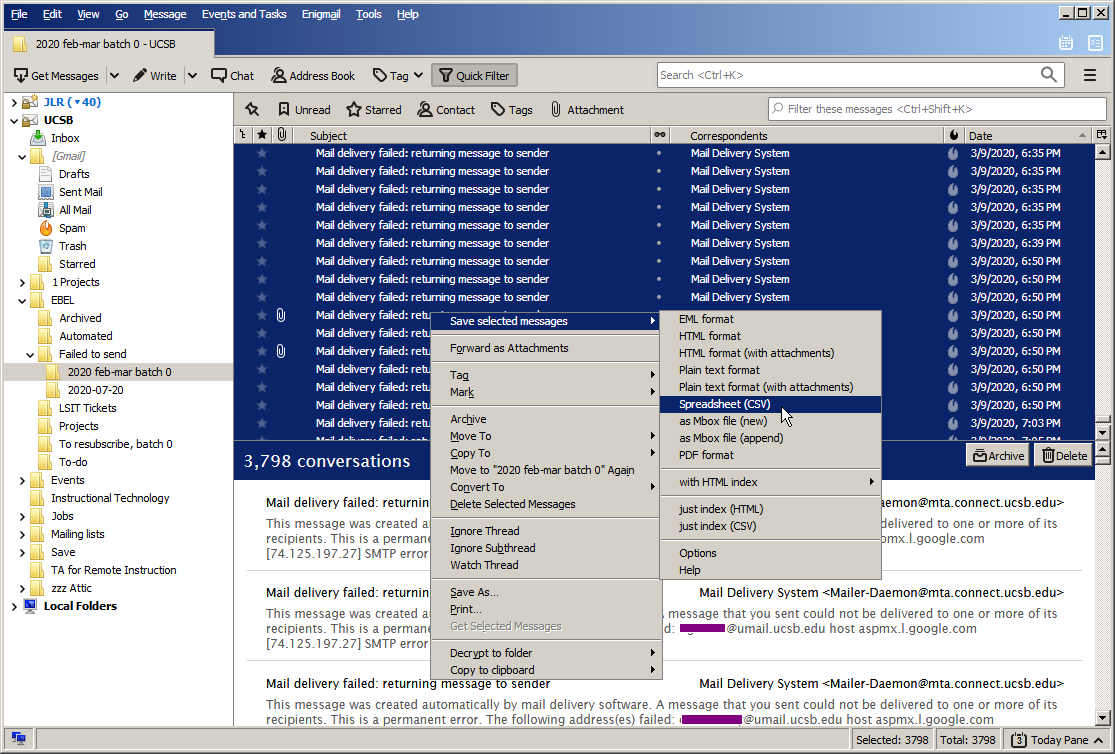
\includegraphics[height=7cm]{email-export-as-csv.png}
\end{frame}

\begin{frame}{Open CSV file in gVim}
\begin{itemize}
\item The line in the brown box is one-to-one with the set of emails
\item We will extract the email address from this line in each returned email
\end{itemize}
\vspace{0.25cm}
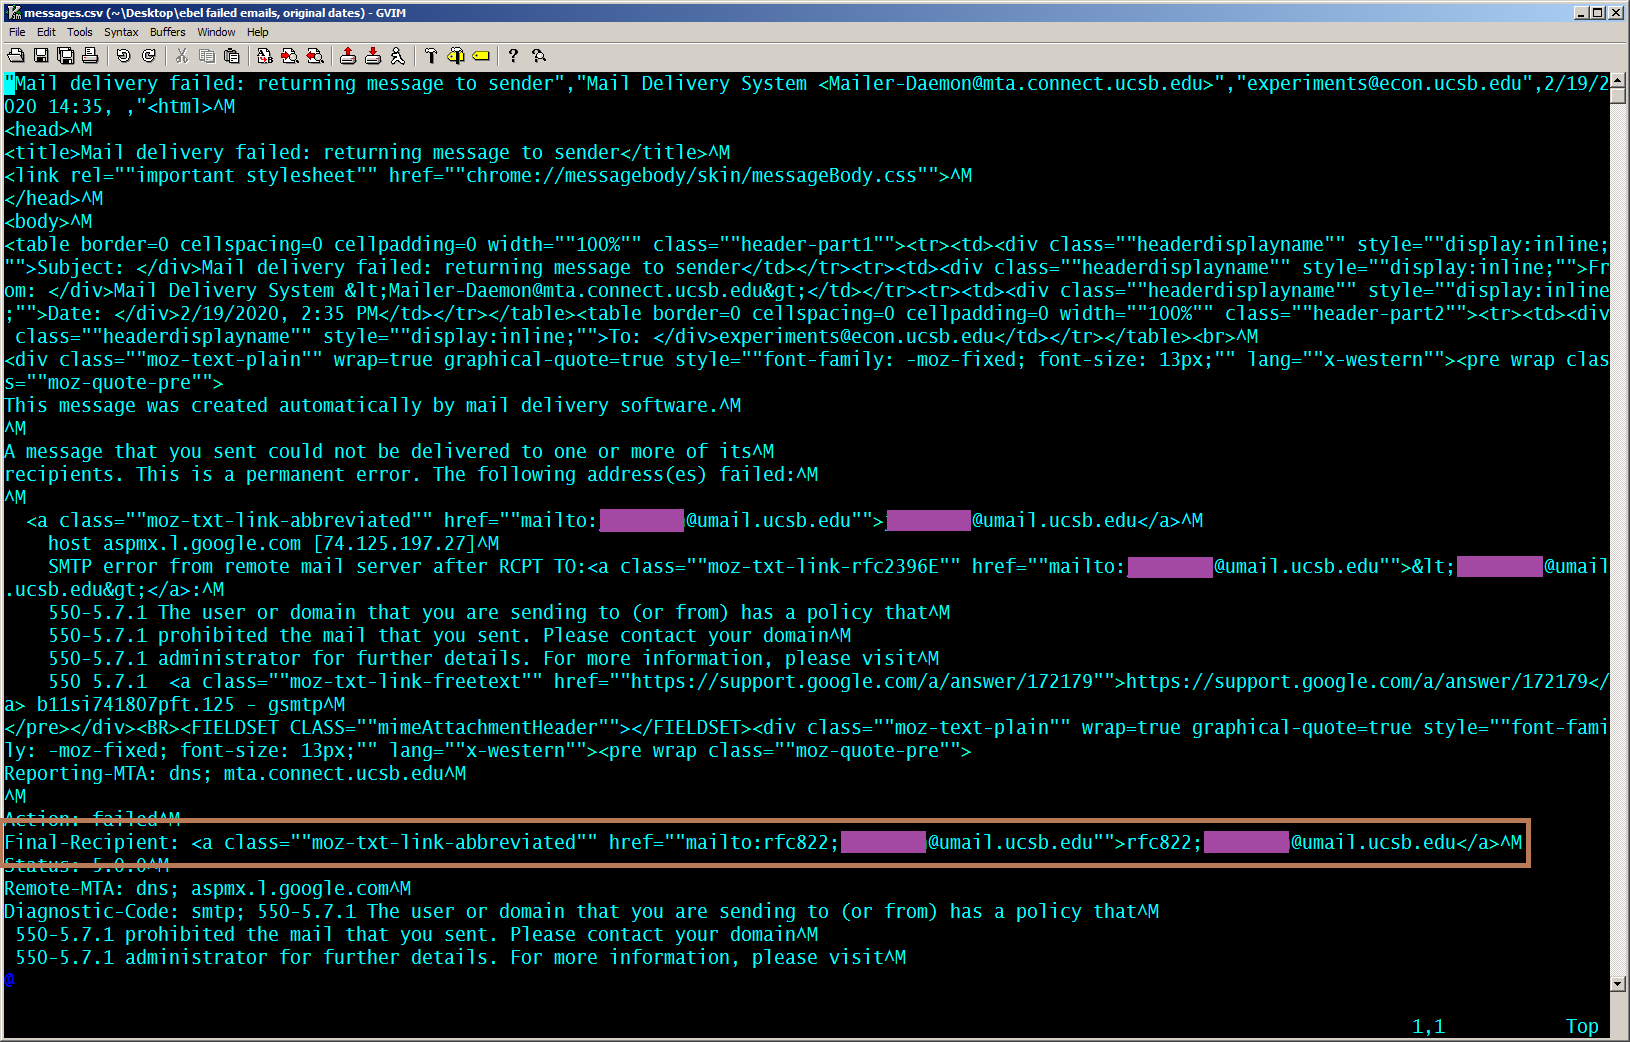
\includegraphics[height=7cm]{vim-csv-0.png}
\end{frame}

\begin{frame}{Regular expressions in gVim}
\begin{itemize}
\item Type a colon (\textcolor{blue}{\texttt{:}}) to begin a command
\item Type command \textcolor{blue}{\texttt{\%g!/Final-Recipient:/d}}
\item Press return to execute
\vspace{0.25cm}
\item Explanation:
\begin{itemize}
\item Globally (\textcolor{blue}{\texttt{\%g}}), if not (\textcolor{blue}{\texttt{!}}) match \textcolor{blue}{\texttt{Final-Recipient:}}, delete (\textcolor{blue}{\texttt{d}})
\end{itemize}
\end{itemize}
\vspace{0.25cm}
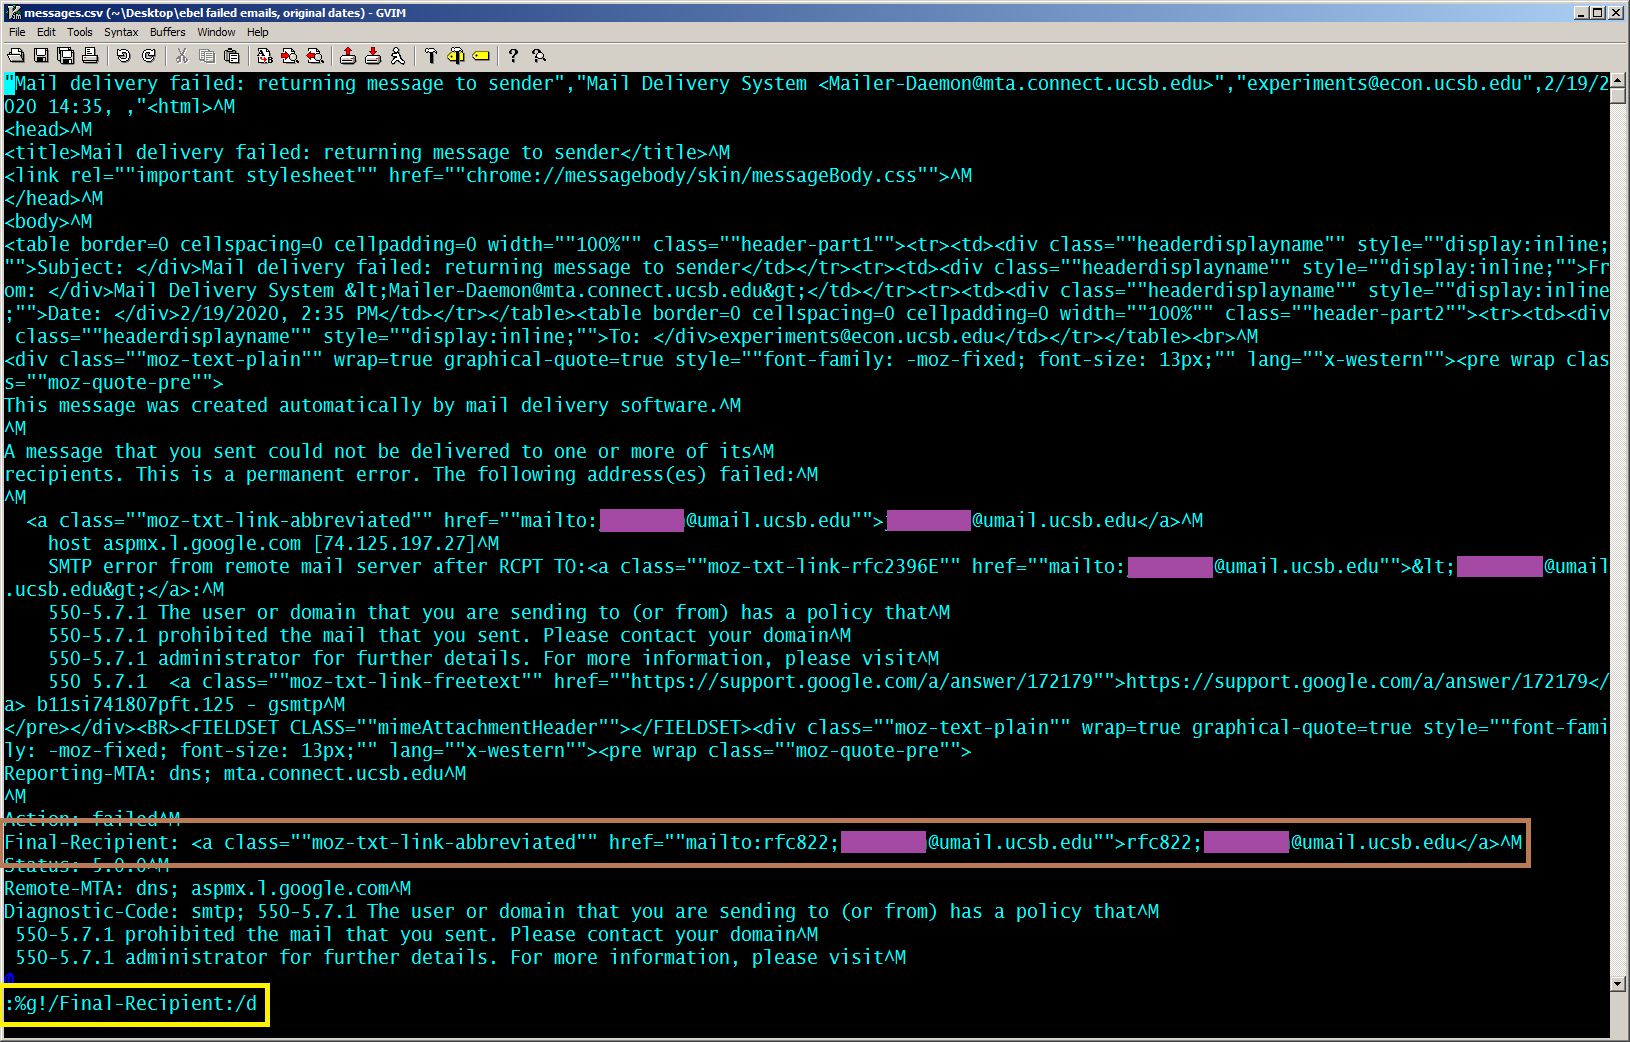
\includegraphics[height=3cm,trim=0 0 0 16cm,clip]{vim-csv-1.png}
\end{frame}

\begin{frame}{Regular expressions in gVim}
\begin{itemize}
\item Here is the result
\end{itemize}
\vspace{0.25cm}
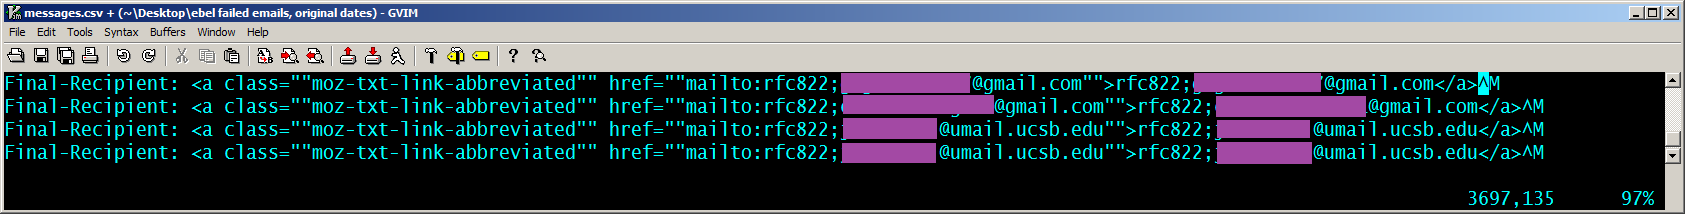
\includegraphics[width=\textwidth]{vim-csv-2.png}
\end{frame}

\begin{frame}{Regular expressions in gVim}
\begin{itemize}
\item Type a colon (\textcolor{blue}{\texttt{:}}) to begin a command
\item Type command \textcolor{blue}{\texttt{\%s/Final-Recipient:.*""mailto:rfc822;\char`\\(.*\char`\\)"".*/\char`\\1/g}}
\item Press return to execute
\vspace{0.25cm}
\item Explanation:
\begin{itemize}
\item Search (\texttt{\textcolor{blue}{\%s}}) for \\ \texttt{\textcolor{blue}{Final-Recipient:\textcolor{violet}{.*}""mailto:rfc822;\textcolor{red}{\char`\\(}\textcolor{violet}{.*}\textcolor{red}{\char`\\)}""\textcolor{violet}{.*}}} \\ and replace it with \texttt{\textcolor{red}{\char`\\1}} globally (\texttt{\textcolor{blue}{g}})
\item \texttt{\textcolor{violet}{.*}} matches any number of characters
\item \texttt{\textcolor{red}{\char`\\(}} and \texttt{\textcolor{red}{\char`\\)}} group characters subsequently recalled as \texttt{\textcolor{red}{\char`\\1}} (the first group)
\end{itemize}
\end{itemize}
\vspace{0.25cm}
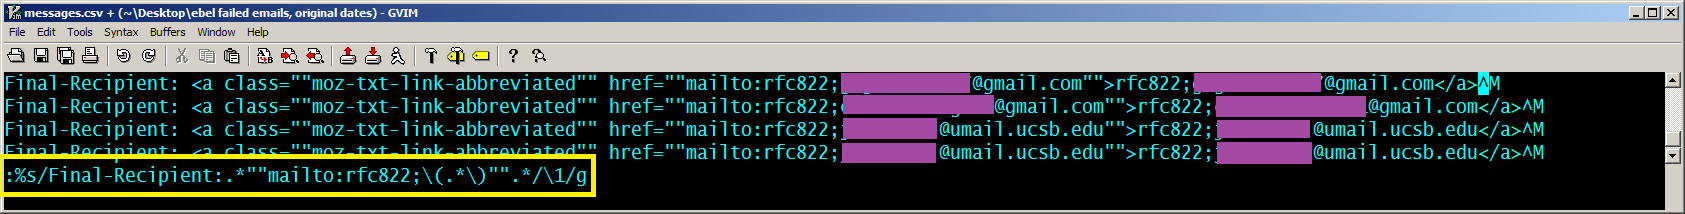
\includegraphics[width=\textwidth]{vim-csv-3.png}
\end{frame}

\begin{frame}{Resultant file of undeliverable email addresses}
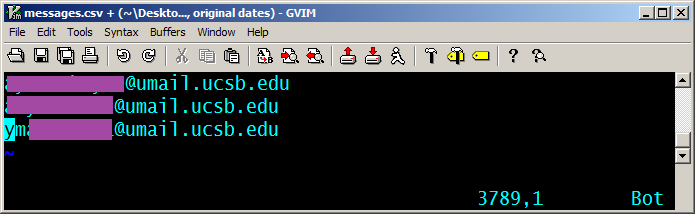
\includegraphics[height=1.5cm]{vim-csv-4.png}
\vspace{0.25cm}
\begin{itemize}
\item Save and exit gVim with \textcolor{blue}{\texttt{:x}} and return
\item Use Unix-like commands to count the number of lines:\\
\texttt{\textcolor{violet}{\$} \textcolor{blue}{cat messages.csv | wc -l}} \\
\textcolor{violet}{\texttt{3789}}
\item Also find how many lines are unique:\\
\texttt{\textcolor{violet}{\$} \textcolor{blue}{sort -u messages.csv | wc -l}}\\
\textcolor{violet}{\texttt{709}}
\item Okay, many duplicates here.
\item Sort the lines, keep only unique lines, and pipe to a new file:\\
\texttt{\textcolor{violet}{\$} \textcolor{blue}{sort -u messages.csv > messages-unique.csv}}
\item Move the resultant file to the same directory as our utility script
\end{itemize}
\end{frame}

\begin{frame}{Using the PHP utility script}
\begin{itemize}
\item The script reads your CSV file and populates an HTML form
\item The form will post to the ORSEE web address you specify
\item Make sure you login to ORSEE so that the search query works!
\vspace{0.25cm}
\item Use the \emph{maxrows} and \emph{skiprows} variables to select specific rows
\item ORSEE can only accept 1000 form variables at once (assuming default PHP configuration on the ORSEE server), so keep $\text{maxrows}<248$
\vspace{0.25cm}
\item An example:
\begin{itemize}
\item Suppose I have 620 email addresses in my CSV file
\item Choosing $\text{maxrows}=200$ and $\text{skiprows}=0$ obtains rows 1--200
\item Choosing $\text{maxrows}=200$ and $\text{skiprows}=200$ obtains rows 201--400
\item Choosing $\text{maxrows}=220$ and $\text{skiprows}=400$ obtains rows 401--620
\item These three searches will span my entire list of 620 email addresses
\end{itemize}
\end{itemize}
\end{frame}

\begin{frame}{PHP utility script}
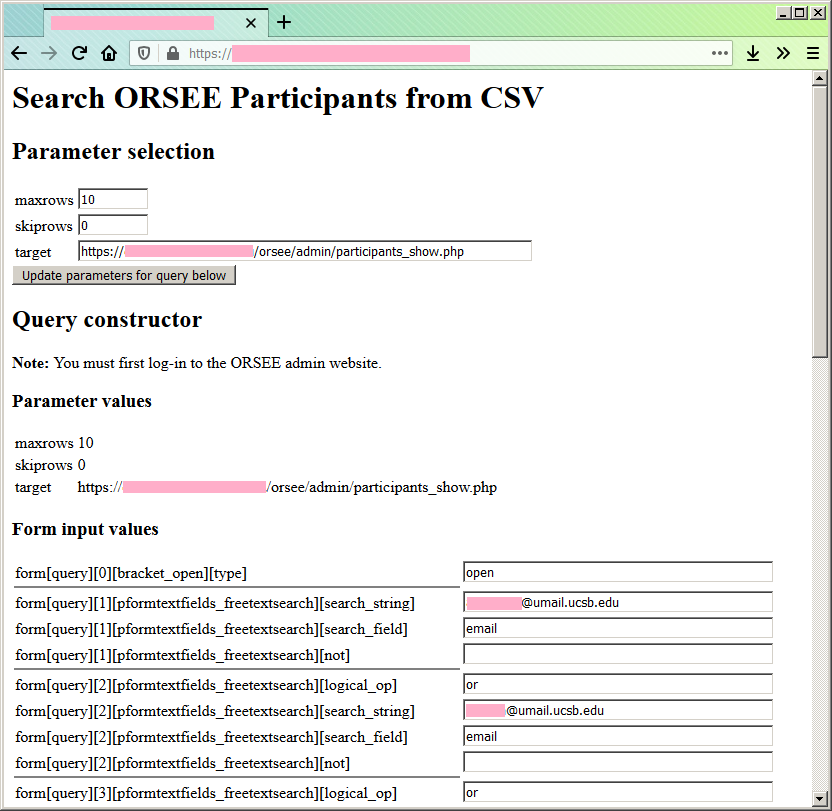
\includegraphics[height=8cm]{web-utility-script.png}
\end{frame}

\begin{frame}{ORSEE search results}
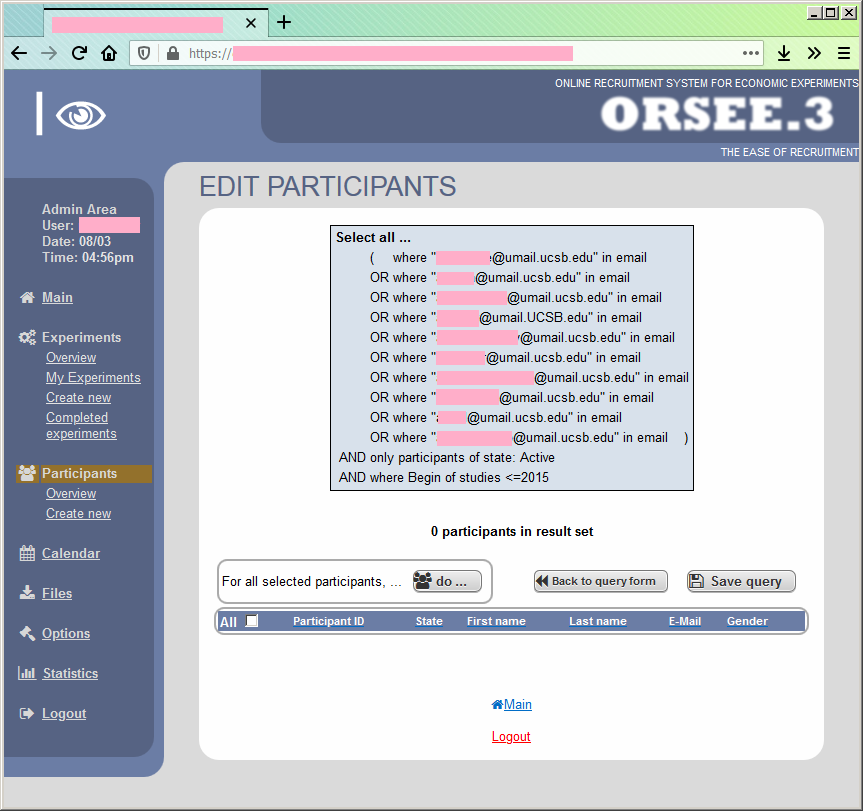
\includegraphics[height=8cm]{orsee-search.png}
\end{frame}

\end{document}
